% Autor: Kryštof Glos

\chapter{Úvod}
Procedurálně vytvářený obsah v herním průmyslu je velmi důležitou součástí her už po několik let. Mnoho her postavených na této vlastnosti už se prosadilo na trhu a stále více se uplatňuje. Náhodné vytváření obsahu se používá například na tvoření herních map, věcí v místnosti, skládání různých dopředu vytvořených místností tak aby vznikla jedinečná mapa, zkrátka skoro všude. 

Hlavním důvodem používání náhodně vytvořeného obsahu je možnost opakovaného hraní stejné hry, bez toho aby se hra stala nezáživnou. V budoucnu se procedurální generování rozhodně neztratí a naopak se bude ještě více využívat v různých odvětvích. Cíl této práce je vytvořit jedinečnou 2D hru z pohledu z hora, která právě takové náhodné vytváření bude používat. Hra je o přežití a ovládání skupiny domorodců a nastolení míru na ostrově. V kapitole \ref{Teorie} je detailně popsáno náhodné generování a různé metody,v kapitole \ref{solution} je vysvětleno jaké způsoby budou nejlepší k řešení, jak byla práce naplánována a proč. V kapitole \ref{realization} je popsaný způsob jakým byla hra řešena, použité metody a jejich význam.

\chapter{Teorie} 
\label{Teorie}
Ve světě her jsou dvě možnosti jak přistupovat ke tvoření obsahu, jedním z těchto způsobů je tradiční nebo také mechanické. \hyperref[traditional]{Mechanické generování} je nejjednodušší, ale také nejpracnější. Další možností vytváření obsahu je pomocí metod implementující náhodné, nebo také \hyperref[procedural]{procedurální generování obsahu}. (anglicky Procedural Generation dále jen PG) je složitější na implementaci, avšak jakmile je implementované tak už žádné navrhování úrovní není třeba, takové úrovně však mohou mít chyby pokud nejsou správně ošetřeny. (například nedostupné místnosti, rostlina na vodě, atd.)

Hry které mají pouze dvě dimenze se nazývají 2D. (z anglického two dimensions) Je mnoho žánrů 2D her, RPG (role playing game) hry na hrdiny s příběhem, strategií, Co-op (kooperační) které jsou postavené na spolupráci více hráčů, survival (hry o přežití), colony-sim (z anglického colonization simulation) které mají simulovat kolonizaci ovládanou hráčem a tak dále. Tato bakalářská práce se zabývá hrou žánru colony-sim. Je mnoho způsobů jak vyvíjet takovou hru, nejčastěji se používají takzvané \hyperref[enginy]{herní enginy}, které takové vyvíjení hry ulehčují a jsou na to stavěné.


\section{Způsoby generování obsahu}
V této části porovnáme mechanické generování obsahu s procedurálním, vysvětlíme co je lepší kdy použít a jaké známe metody pro procedurální generování. Následující tři body popisují faktory, které je třeba zvážit při rozhodování, zda bude využita nějaká procedurální metoda na generování, nebo bude lepší použít manuální design úrovní a obsahu:
\begin{description}
	\item[Žánr tvořené hry] Při vytváření například takové FPS hry, u které záleží hlavně na ovládání a souboji hráče proti hráči, není třeba vytvářet mapy a další obsah procedurálně. Většinou stačí vytvořit například pouze jednu úroveň a na to není potřeba požívat procedurální generování. Při hrách které závisí na okolí, surovinách a přežití kde každá okolnost nějak ovlivňuje hráče, už procedurální generování hraje větší roli
	\item[Opakovaná hratelnost] Některé hry jsou dělané tak že čím déle hráč hraje stejnou úroveň(anglicky level) tím více se zlepšuje a je za to například odměňován je právě manuální tvoření úrovní lepší než procedurální. Naopak u jiných her, které mají úrovně procedurálně generované, většinou hráč danou úroveň zvládne, pokračuje na další a nepředpokládá se že se k ní bude ještě vracet.
	\item[Aspekt designu hry] Jestliže hra závisí z velké části na jedné úrovni s jejími mechanikami, vlastnostmi a obsahem, pak je lepší ji vytvářet mechanicky a doladit všechny vlastnosti a interakce s hráčem.
\end{description}


\subsection{Mechanické generování obsahu}
\label{traditional}
Mechanický typ generování je jedním z nejobvyklejších tvoření obsahu ve hrách. Používá se převážně v žánrech, jako je RPG (Role Play Game), RTS(Real Time Strategy) a další, ve kterých pozice objektů a struktura mapy hraje velkou roli a bez lidské tvorby by nebylo dosaženo potřebných výsledků. Toto tvoření lze interpretovat jako proces u něhož se návrhář za pomoci různých nástrojů, které postupně aplikuje, snaží dosáhnout požadovaného výsledku. Jde tedy o metodu ručního vytváření obsahu kde designér, nebo grafik navrhuje a postupně vytváří úroveň, či jinou část hry tak, aby vyhovovala potřebám.
	
Proces takového vytváření obsahu pro hry se dá zjednodušeně představit na příkladu. Uvažujme například truhláře vyrábějícího stůl, který také používá různé nástroje na zhotovení nábytku. Aplikováním těchto nástrojů na materiál postupně vytváří výsledný stůl. Nástroje a suroviny, které si na počátku celého procesu vybral, určí možné výsledky, takže výsledkem jeho práce nemůže být třeba obraz.

Díky tomuto přístupu nehrozí nesrovnalosti ve výsledku, například se nemůže stát že určitá část mapy bude nedostupná, nebo úplně nesmyslná. Další výhodou je, že výsledek bude přesně takový jak byl naplánovaný, avšak takovéto tvoření je u větších her, kde je nutná opětovná hratelnost, velmi časově náročné.

\subsection{Procedurální generování obsahu}
\label{procedural}
Roden and Parberry \cite{FromArtistry} pojmenovávají tento druh algoritmů \textit{amplifikační algoritmy (amplification algorithms)}, přijímají menší množství vstupních informací, které zpracují a vracejí větší objem dat na výstupu. Hendrikx et al. \cite{Hendrikx} pojímají procedurální generování jako alternativu k mechanickému navrhování obsahu, ale kladou důraz na zdokonalování a přidávání parametrů umožňujících zásah návrháře do takto vygenerovaných objektů.

Tento typ vytváření obsahu se používá ve více žánrech, ale asi nejznámější z hlediska generování map je Roguelike, kde každá nová hra má unikátní náhodnou mapu. PG se ovšem nepoužívá pouze na generování map, ale také na vytváření objektů, jako jsou stromy, textury, animace a další. Procedurální generování obsahu není to stejné jako, jak se mnozí domnívají, náhodné generování obsahu.

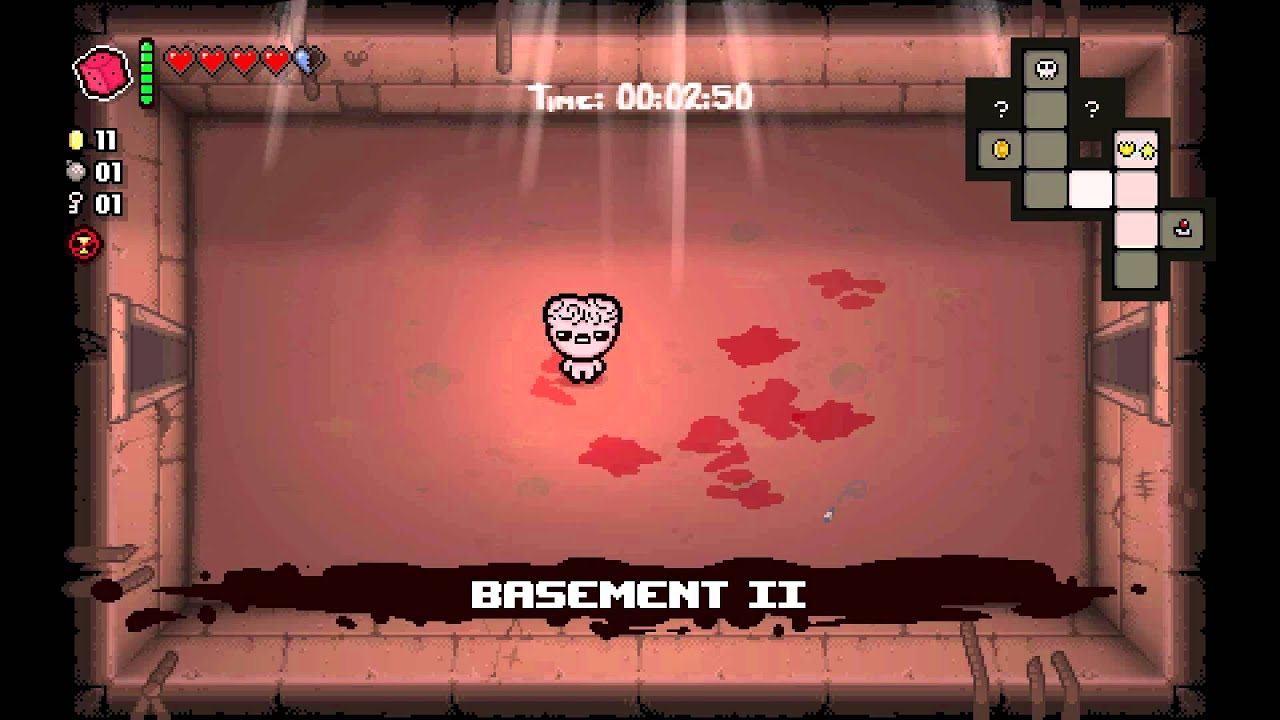
\includegraphics[scale=0.3]{obrazky-figures/BindingOfIsaac.jpg}

V zásadě je to proces obrácený jak u mechanického generování obsahu. Uživatel sice stále definuje různé nástroje, které jsou použity pro vytváření obsahu, ale nikoli pro své vlastní použití, ale naopak je vytváří pro algoritmus. Uživatel dále určuje pravidla podle kterých se generátor musí řídit tak, aby se dobral kýženého výsledku.

\subsubsection{Příklad procedurálního generování lesů}
\label{proceduralExample}
Pro lepší představu uvedu příklad. Program má funkci procedurálního generátoru lesů na mapě, cílem tohoto programu je náhodně naskládat stromy s rozumnými rozestupy od sebe. Pomocí mechanického generování obsahu by designér jednoduše přidával modely stromů do té doby, dokud by mapa neodpovídala představám návrháře a nesplňovala by potřeby herního designu. V případě procedurálního generování, je nutné definovat nástroje, což je v tomto příkladě schopnost přidávat stromy na mapu a pravidla, jako například kolik stromů je potřeba aby algoritmus vysázel, kam program může jednotlivé stromy pokládat a jaké jsou minimální rozestupy mezi nimi. Pravidla a nástroje nám tím pádem jednoznačně definují množinu potenciálních výsledku.

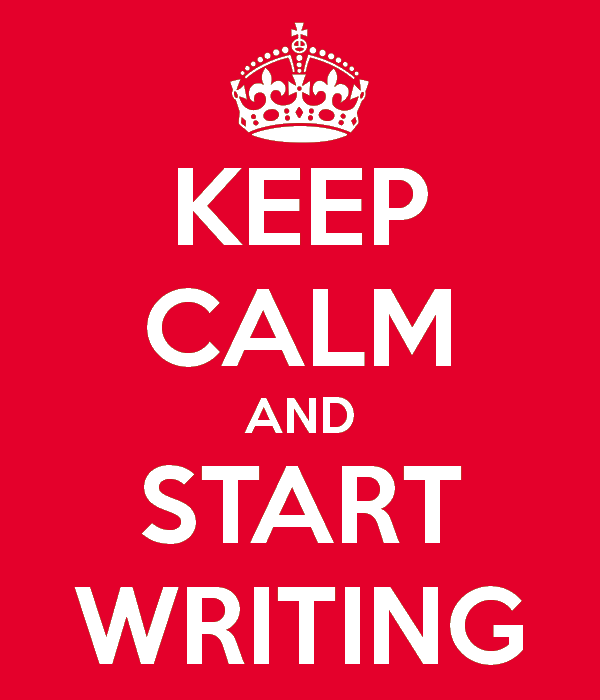
\includegraphics[scale=0.3]{obrazky-figures/keep-calm.png}
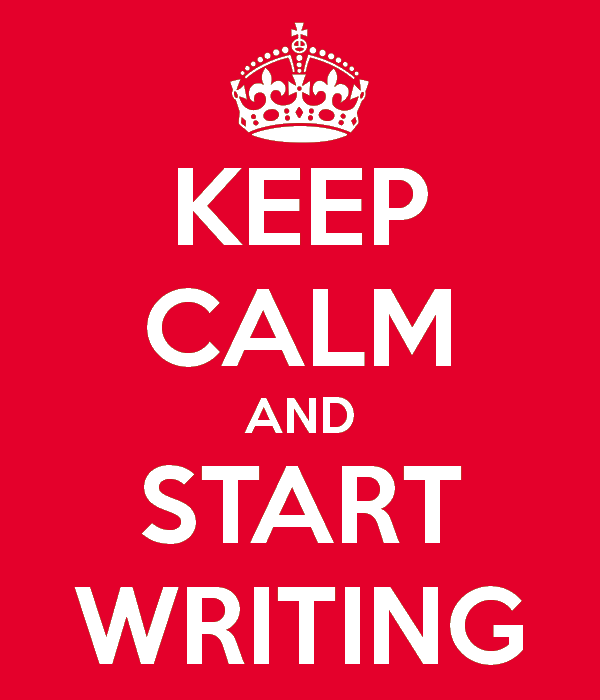
\includegraphics[scale=0.3]{obrazky-figures/keep-calm.png}

\todo{dva obrázky, jeden se stromy moc u sebe a druhý lepší}

\subsubsection{Známé metody na procedurální generování}
\label{metody}
Algoritmů na generování obsahu existuje mnoho, každý používá jiné nástroje, ale všechny se musí podrobovat pravidlům která stanovuje programátor a podle kterých se řídí. Velmi silně záleží ovšem na tom, čeho chceme docílit. Pro generování například vegetace, se používají jiné metody, než třeba pro vytváření krajiny.

\todo{informace o všemožných známých metodách procedurálního generování}

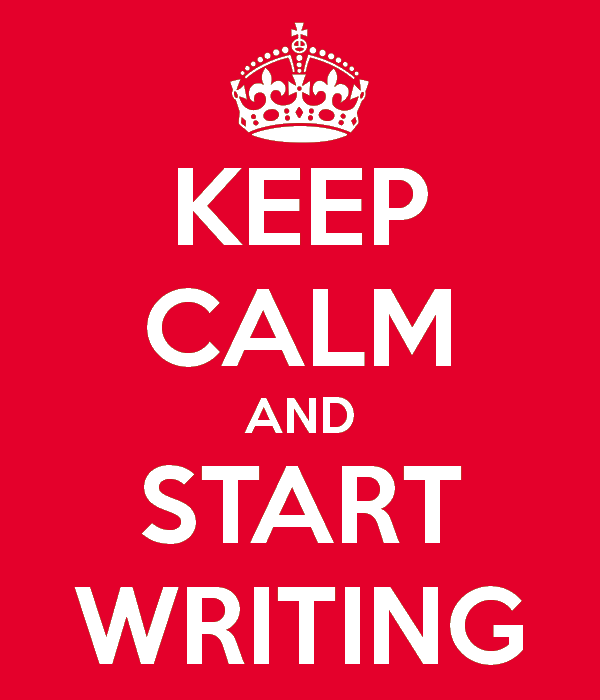
\includegraphics[scale=0.3]{obrazky-figures/keep-calm.png}

\textcolor{gray}{\blindtext[10]}


\subsubsection{Porovnání metod}
\todo{porovnání jednotlivých metod}
\textcolor{gray}{\blindtext[8]}

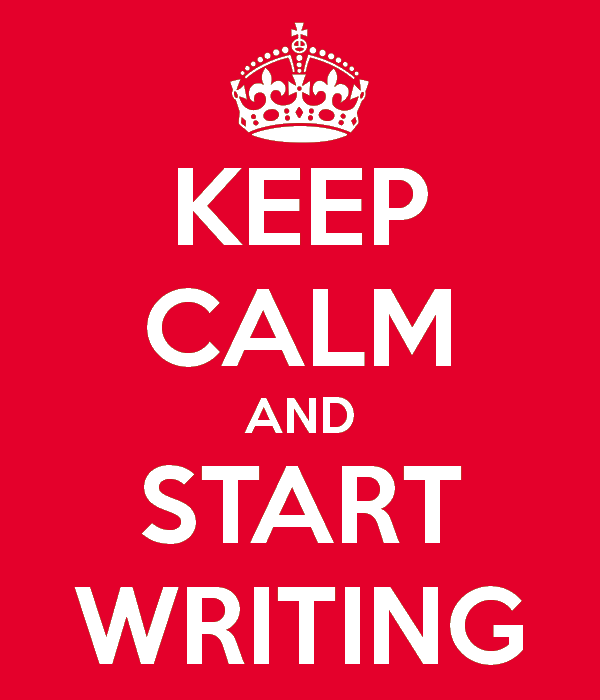
\includegraphics[scale=0.3]{obrazky-figures/keep-calm.png}

\textcolor{gray}{\blindtext[23]}


\section{2D hry}

\todo{popis hry}
\textcolor{gray}{\blindtext[18]}
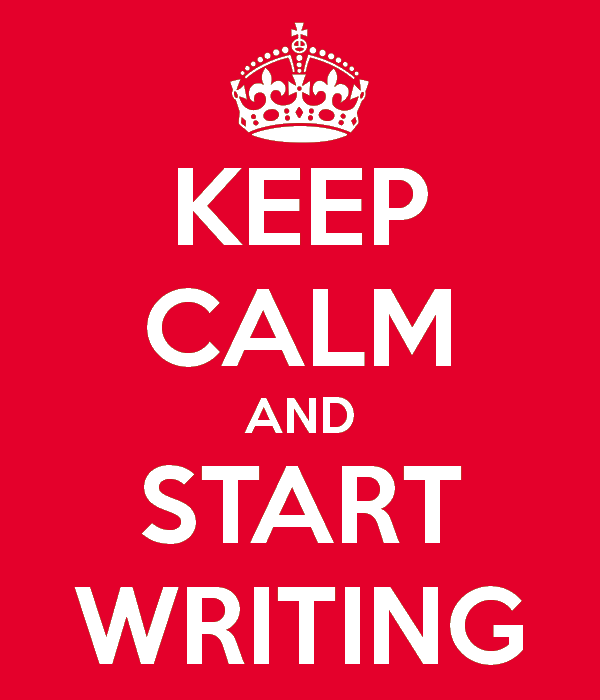
\includegraphics[scale=0.3]{obrazky-figures/keep-calm.png}

\subsection{Enginy na vývoj her}
\label{enginy}
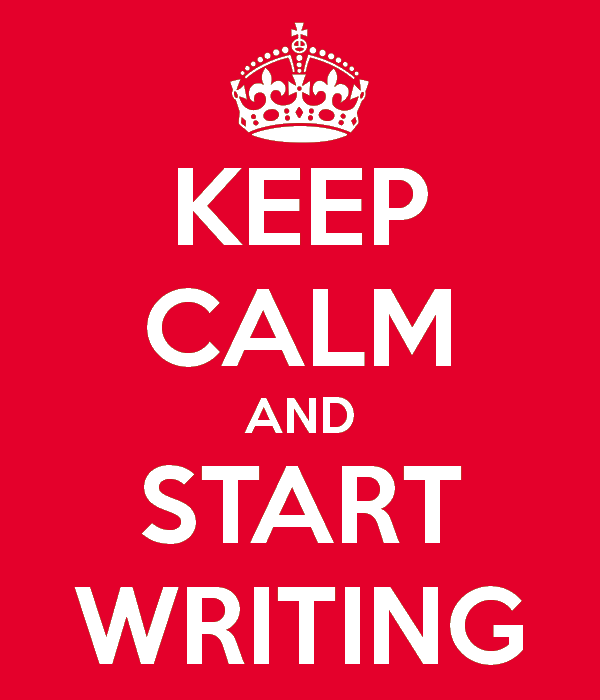
\includegraphics[scale=0.3]{obrazky-figures/keep-calm.png}

\textcolor{gray}{\blindtext[18]}

\chapter{Návrh řešení}
\label{solution}
\textcolor{gray}{\blindtext[2]}
\textcolor{gray}{\blindtext[46]}

\section{Vybraná metoda generování}
\todo{podrobnější popis metody, výhody, nevýhody}
\textcolor{gray}{\blindtext[46]}

\chapter{Realizace, experimenty a vyhodnocení}
\label{realization}
\textcolor{gray}{\blindtext[94]}

\chapter{Závěr}
\label{end}
\textcolor{gray}{\blindtext[4]}